% Options for packages loaded elsewhere
\PassOptionsToPackage{unicode}{hyperref}
\PassOptionsToPackage{hyphens}{url}
\PassOptionsToPackage{dvipsnames,svgnames,x11names}{xcolor}
%
\documentclass[
  letterpaper,
  DIV=11,
  numbers=noendperiod,
  oneside]{scrreprt}

\usepackage{amsmath,amssymb}
\usepackage{lmodern}
\usepackage{iftex}
\ifPDFTeX
  \usepackage[T1]{fontenc}
  \usepackage[utf8]{inputenc}
  \usepackage{textcomp} % provide euro and other symbols
\else % if luatex or xetex
  \usepackage{unicode-math}
  \defaultfontfeatures{Scale=MatchLowercase}
  \defaultfontfeatures[\rmfamily]{Ligatures=TeX,Scale=1}
\fi
% Use upquote if available, for straight quotes in verbatim environments
\IfFileExists{upquote.sty}{\usepackage{upquote}}{}
\IfFileExists{microtype.sty}{% use microtype if available
  \usepackage[]{microtype}
  \UseMicrotypeSet[protrusion]{basicmath} % disable protrusion for tt fonts
}{}
\makeatletter
\@ifundefined{KOMAClassName}{% if non-KOMA class
  \IfFileExists{parskip.sty}{%
    \usepackage{parskip}
  }{% else
    \setlength{\parindent}{0pt}
    \setlength{\parskip}{6pt plus 2pt minus 1pt}}
}{% if KOMA class
  \KOMAoptions{parskip=half}}
\makeatother
\usepackage{xcolor}
\usepackage[left=1in,marginparwidth=2.0666666666667in,textwidth=4.1333333333333in,marginparsep=0.3in]{geometry}
\setlength{\emergencystretch}{3em} % prevent overfull lines
\setcounter{secnumdepth}{-\maxdimen} % remove section numbering
% Make \paragraph and \subparagraph free-standing
\ifx\paragraph\undefined\else
  \let\oldparagraph\paragraph
  \renewcommand{\paragraph}[1]{\oldparagraph{#1}\mbox{}}
\fi
\ifx\subparagraph\undefined\else
  \let\oldsubparagraph\subparagraph
  \renewcommand{\subparagraph}[1]{\oldsubparagraph{#1}\mbox{}}
\fi


\providecommand{\tightlist}{%
  \setlength{\itemsep}{0pt}\setlength{\parskip}{0pt}}\usepackage{longtable,booktabs,array}
\usepackage{calc} % for calculating minipage widths
% Correct order of tables after \paragraph or \subparagraph
\usepackage{etoolbox}
\makeatletter
\patchcmd\longtable{\par}{\if@noskipsec\mbox{}\fi\par}{}{}
\makeatother
% Allow footnotes in longtable head/foot
\IfFileExists{footnotehyper.sty}{\usepackage{footnotehyper}}{\usepackage{footnote}}
\makesavenoteenv{longtable}
\usepackage{graphicx}
\makeatletter
\def\maxwidth{\ifdim\Gin@nat@width>\linewidth\linewidth\else\Gin@nat@width\fi}
\def\maxheight{\ifdim\Gin@nat@height>\textheight\textheight\else\Gin@nat@height\fi}
\makeatother
% Scale images if necessary, so that they will not overflow the page
% margins by default, and it is still possible to overwrite the defaults
% using explicit options in \includegraphics[width, height, ...]{}
\setkeys{Gin}{width=\maxwidth,height=\maxheight,keepaspectratio}
% Set default figure placement to htbp
\makeatletter
\def\fps@figure{htbp}
\makeatother

\KOMAoption{captions}{tableheading}
\makeatletter
\makeatother
\makeatletter
\makeatother
\makeatletter
\@ifpackageloaded{caption}{}{\usepackage{caption}}
\AtBeginDocument{%
\ifdefined\contentsname
  \renewcommand*\contentsname{Table of contents}
\else
  \newcommand\contentsname{Table of contents}
\fi
\ifdefined\listfigurename
  \renewcommand*\listfigurename{List of Figures}
\else
  \newcommand\listfigurename{List of Figures}
\fi
\ifdefined\listtablename
  \renewcommand*\listtablename{List of Tables}
\else
  \newcommand\listtablename{List of Tables}
\fi
\ifdefined\figurename
  \renewcommand*\figurename{Figure}
\else
  \newcommand\figurename{Figure}
\fi
\ifdefined\tablename
  \renewcommand*\tablename{Table}
\else
  \newcommand\tablename{Table}
\fi
}
\@ifpackageloaded{float}{}{\usepackage{float}}
\floatstyle{ruled}
\@ifundefined{c@chapter}{\newfloat{codelisting}{h}{lop}}{\newfloat{codelisting}{h}{lop}[chapter]}
\floatname{codelisting}{Listing}
\newcommand*\listoflistings{\listof{codelisting}{List of Listings}}
\makeatother
\makeatletter
\@ifpackageloaded{caption}{}{\usepackage{caption}}
\@ifpackageloaded{subcaption}{}{\usepackage{subcaption}}
\makeatother
\makeatletter
\@ifpackageloaded{tcolorbox}{}{\usepackage[many]{tcolorbox}}
\makeatother
\makeatletter
\@ifundefined{shadecolor}{\definecolor{shadecolor}{rgb}{.97, .97, .97}}
\makeatother
\makeatletter
\@ifpackageloaded{sidenotes}{}{\usepackage{sidenotes}}
\@ifpackageloaded{marginnote}{}{\usepackage{marginnote}}
\makeatother
\makeatletter
\makeatother
\ifLuaTeX
  \usepackage{selnolig}  % disable illegal ligatures
\fi
\IfFileExists{bookmark.sty}{\usepackage{bookmark}}{\usepackage{hyperref}}
\IfFileExists{xurl.sty}{\usepackage{xurl}}{} % add URL line breaks if available
\urlstyle{same} % disable monospaced font for URLs
\hypersetup{
  pdftitle={Artificial Intelligence},
  pdfauthor={Fred Guth},
  colorlinks=true,
  linkcolor={blue},
  filecolor={Maroon},
  citecolor={Blue},
  urlcolor={Blue},
  pdfcreator={LaTeX via pandoc}}

\title{Artificial Intelligence}
\usepackage{etoolbox}
\makeatletter
\providecommand{\subtitle}[1]{% add subtitle to \maketitle
  \apptocmd{\@title}{\par {\large #1 \par}}{}{}
}
\makeatother
\subtitle{`I visualise a time when we will be to robots what dogs are to
humans,\ldots{} and I am rooting for the machines.' --- Claude Shannon}
\author{Fred Guth}
\date{2022-09-30}

\begin{document}
\maketitle
\ifdefined\Shaded\renewenvironment{Shaded}{\begin{tcolorbox}[frame hidden, boxrule=0pt, breakable, enhanced, interior hidden, borderline west={3pt}{0pt}{shadecolor}, sharp corners]}{\end{tcolorbox}}\fi

\renewcommand*\contentsname{Table of contents}
{
\hypersetup{linkcolor=}
\setcounter{tocdepth}{2}
\tableofcontents
}
This chapter defines artificial intelligence, presents the
epistemological differences of intelligent agents in history, and
discusses their consequences to machine learning theory.

\hypertarget{artificial-intelligence}{%
\section{Artificial Intelligence}\label{artificial-intelligence}}

\protect\hypertarget{def-ai}{}{} \textbf{AI} is the branch of Computer
Science that studies general principles of intelligent agents and how to
construct them~(\textbf{russell:2010?}).

This definition uses the terms \emph{intelligence} and \emph{intelligent
agents}, so let us start from them.

\hypertarget{what-is-intelligence}{%
\subsection{What is intelligence?}\label{what-is-intelligence}}

Despite a long history of research, there is still no consensual
definition of intelligence.\sidenote{\footnotesize For a list with 70 definitions of
  intelligence, see~.} Whatever it is, though, humans are particularly
proud of it. We even call our species \emph{homo sapiens}, as
intelligence was an intrinsic human characteristic.

In this dissertation:

\protect\hypertarget{def-intelligence}{}{\textbf{Intelligence}} is the
ability to predict a course of action to achieve success in specific
goals.

\hypertarget{intelligent-agents}{%
\subsection{Intelligent Agents}\label{intelligent-agents}}

Under our generous definition, intelligence is not limited to humans. It
applies to any agent\sidenote{\footnotesize An agent is anything that perceives its
  environment and acts on it.}: animal or machine. For example, a
bacteria can perceive its environment through chemical signals, process
them, and then produce chemicals to signal other bacteria. An
air-conditioning can observe temperature changes, know its state, and
adapt its functioning, turning off if it is cold or on if it is hot ---
\emph{intelligence exempts understanding}. The air-conditioning does not
comprehend what it is doing. The same way a calculator does not know
arithmetics.

\hypertarget{a-strange-inversion-of-reasoning}{%
\subsection{A strange inversion of
reasoning}\label{a-strange-inversion-of-reasoning}}

This competence without comprehension is what the philosopher Daniel
Dennett calls \emph{Turing's strange inversion of
reasoning}\sidenote{\footnotesize In his work, Turing discusses if computers can
  ``think'', meaning to examine if they can perform indistinguishably
  from the way thinkers do.}\protect\hypertarget{turing_strange_inversion}{}{}.
The idea of a \emph{strange inversion} comes from one of Darwin's
19\textsuperscript{th}-century critics ((\textbf{mackenzie:1868?}) as
cited by~(\textbf{dennett:2009?})):

\begin{quote}
\emph{In the theory with which we have to deal, Absolute Ignorance is
the artificer; so that we may enunciate as the fundamental principle of
the whole system, that, \textbf{in order to make a perfect and beautiful
machine, it is not requisite to know how to make it}. This proposition
will be found, on careful examination, to express, in condensed form,
the essential purport of the {[}Evolution{]} Theory, and to express in a
few words all Mr Darwin's meaning; who, by \textbf{a strange inversion
of reasoning}, seems to think Absolute Ignorance fully qualified to take
the place of Absolute Wisdom in all of the achievements of creative
skill.} --- Robert MacKenzie\\
\end{quote}

Counterintuitively to (\textbf{mackenzie:1868?}) and many others to this
date, intelligence can emerge from absolute ignorance. Turing's strange
inversion of reasoning comes from the realisation that his automata can
perform calculations by symbol manipulation, proving that it is possible
to build agents that behave intelligently, even if they are entirely
ignorant of the meaning of what they are doing~(\textbf{turing:2007?}).

\hypertarget{dreaming-of-robots}{%
\section{Dreaming of robots}\label{dreaming-of-robots}}

\hypertarget{from-mythology-to-logic}{%
\subsection{From mythology to Logic}\label{from-mythology-to-logic}}

The idea of creating an intelligent agent is perhaps as old as humans.
There are accounts of artificial intelligence in almost any ancient
mythology: Greek, Etruscan, Egyptian, Hindu,
Chinese~(\textbf{mayor:2018?}). For example, in Greek mythology, the
story of the bronze automaton of Talos built by Hephaestus, the god of
invention and blacksmithing, first mentioned around 700 BC.

This interest may explain why, since ancient times, philosophers have
looked for \emph{mechanical} methods of reasoning. Chinese, Indian and
Greek philosophers all developed formal deduction in the first
millennium BC.In particular, Aristotelian syllogism, \emph{laws of
thought}, provided patterns for argument structures to yield irrefutable
conclusions, given correct premises. These ancient developments were the
beginning of the field we now call \emph{Logic}.

\hypertarget{sec-rationalism}{%
\subsection{Rationalism: The Cartesian view of
Nature}\label{sec-rationalism}}

\begin{marginfigure}

{\centering 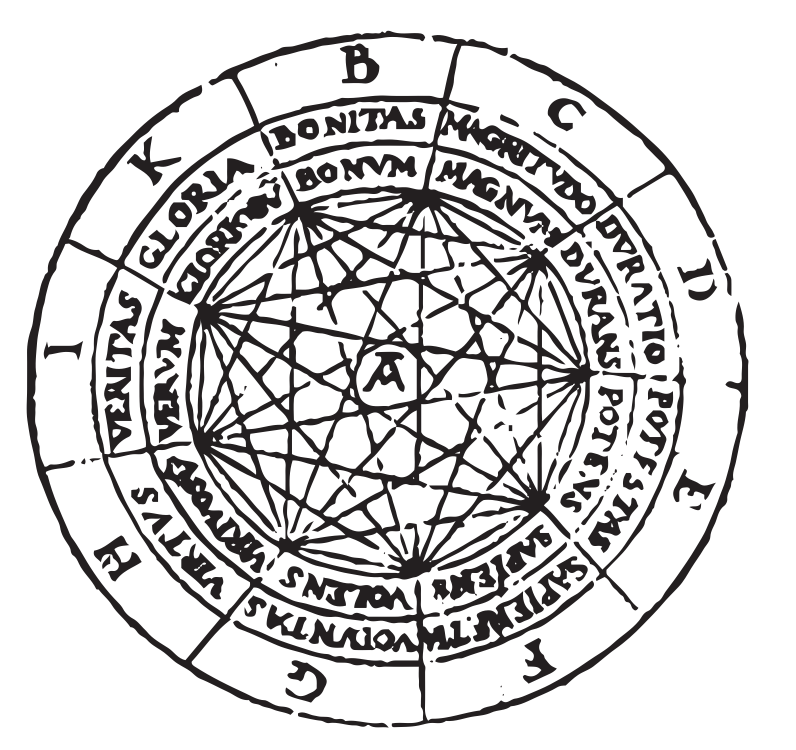
\includegraphics{imgs/ars_magna_disc.png}

}

\caption{\label{fig-ars_magna_disc}Example of one of Lull's Ars Magna's
paper discs.}

\end{marginfigure}

In the 13\textsuperscript{th} century, the Catalan philosopher Ramon
Lull wanted to produce all statements the human mind can think. For this
task, he developed \emph{logic paper machines}, discs of paper filled
with esoteric coloured diagrams that connected symbols representing
statements. Unfortunately, according to~(\textbf{gardner:1959?}), in a
modern reassessment of his work, \emph{``it is impossible, perhaps, to
avoid a strong sense of anticlimax''}~(\textbf{gardner:1959?}). With
megalomaniac self-esteem that suggests psychosis, his delusional sense
of importance is more characteristic of cult founders. On the bright
side, his ideas and books exerted some magic appeal that helped them be
rapidly disseminated through all Europe~(\textbf{gardner:1959?}).

Lull's work greatly influenced Leibniz and Descartes, who, in the
17\textsuperscript{th}century, believed that all rational thought could
be mechanised. This belief was the basis of \textbf{rationalism}, the
epistemic view of the \emph{Enlightenment} that regarded reason as the
sole source of knowledge. In other words, they believed that reality has
a logical structure and that certain truths are \emph{self-evident}, and
all truths can be derived from them.

There was considerable interest in developing artificial languages
during this period. Nowadays, they are called formal languages.

\begin{quote}
\emph{If controversies were to arise, there would be no more need for
disputation between two philosophers than between two accountants. For
it would suffice to take their pencils in their hands, to sit down to
their slates, and to say to each other: \textbf{Let us calculate.}} ---
Gottfried Leibniz
\end{quote}

The rationalist view of the world has had an enduring impact on society
until today. In the 19\textsuperscript{th}century, George Boole and
others developed a precise notation for statements about all kinds of
objects in Nature and their relations. Before them, Logic was
philosophical rather than mathematical. The name of Boole's masterpiece,
\emph{``The Laws of Thought''}, is an excellent indicator of his
Cartesian worldview.

At the beginning of the 20\textsuperscript{th} century, some of the most
famous mathematicians, David Hilbert, Bertrand Russel, Alfred Whitehead,
were still interested in formalism: they wanted mathematics to be
formulated on a solid and complete logical foundation. In particular,
Hilbert's \emph{Entscheidungs Problem} (decision problem) asked if there
were limits to mechanical Logic proofs~(\textbf{chaitin:2006?}).

Kurt Gödel's incompleteness theorem (1931) proved that any language
expressive enough to describe arithmetics of the natural numbers is
either incomplete or inconsistent. This theorem imposes a limit on logic
systems. There will always be truths that will not be provable from
within such languages: there are ``true'' statements that are
undecidable.

Alan Turing brought a new perspective to the \emph{Entscheidungs
Problem}: a function on natural numbers that an algorithm in a formal
language cannot represent cannot be computable~(\textbf{chaitin:2006?}).
Gödel's limit appears in this context as functions that are not
computable, ~no algorithm can decide whether another algorithm will stop
or not (the halting problem). To prove that, Turing developed a whole
new general theory of computation: what is computable and how to compute
it, laying out a blueprint to build computers, and making possible
Artificial Intelligence research as we know it. An area in which Turing
himself was very much invested.

\hypertarget{sec-empiricism}{%
\subsection{Empiricism: The sceptical view of
Nature}\label{sec-empiricism}}

\begin{marginfigure}

{\centering 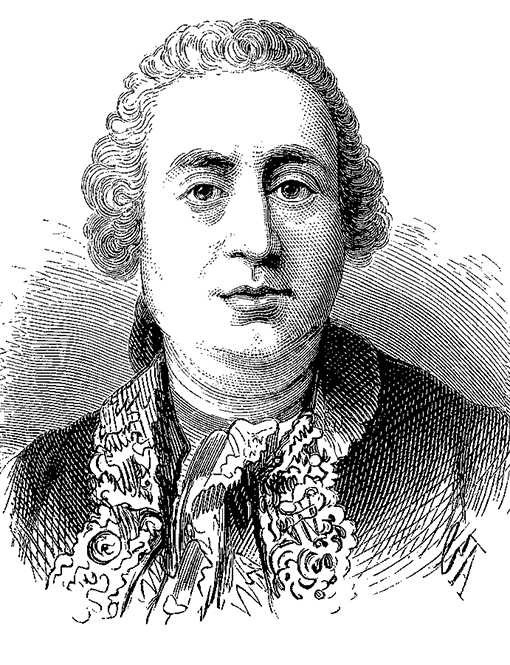
\includegraphics{imgs/hume.png}

}

\caption{\label{fig-hume}David Hume, Scottish Enlightenment philosopher,
historian, economist, librarian and essayist.}

\end{marginfigure}

The response to \textbf{rationalism} was \textbf{empiricism}, the
epistemological view that knowledge comes from sensory experience, our
perceptions of the world. Locke explains this with the peripatetic
axiom\sidenote{\footnotesize This citation is the principle from the Peripatetic
  school of Greek philosophy and is found in Thomas Aquinas' work cited
  by Locke.}: \emph{``there is nothing in the intellect that was not
previously in the senses''}~(\textbf{williams:2020?}). Bacon, Locke and
Hume were great exponents of this movement, which established the
grounds of the scientific method.

David Hume, in particular, presented in the 18\textsuperscript{th}
century a radical empiricist view: reason only does not lead to
knowledge. In~(\textbf{hume:2009?}), Hume distinguishes \emph{relations
of ideas}, propositions that derive from deduction and \emph{matters of
facts}, which rely on the connection of cause and effect through
experience (induction). Hume's critiques, known as \emph{the Problem of
Induction}, added a new slant on the debate of the emerging scientific
method.

From Hume's own words:

\begin{quote}
\emph{The bread, which I formerly eat, nourished me; that is, a body of
such sensible qualities was, at that time, endued with such secret
powers: but does it follow, that other bread must also nourish me at
another time, and that like sensible qualities must always be attended
with like secret powers? The consequence seems nowise necessary.} ---
David Hume
\end{quote}

There is no logic to deduce that the future will resemble the past.
Still, we expect uniformity in Nature. As we see more examples of
something happening, it is \emph{wise} to expect that it will happen in
the future just as it did in the past. There is, however, no
\emph{rationality}\sidenote{\footnotesize \protect\hypertarget{fn:note1}{}{}In the
  philosophical sense.} in this expectation.

Hume explains that we see conjunction repeatedly, ``bread'' and
``nourish'', and we expect \emph{uniformity in Nature}; we hope that
``nourish'' will always follow ``eating bread''; When we fulfil this
expectancy, we misinterpret it as causation. In other words, we
\emph{project} causation into phenomena. Hume explained that this
connection does not exist in Nature. We do not ``see causation''; we
create it.

This projection is \emph{Hume's strange inversion of
reasoning}~(\textbf{huebner:2017?}): We do not like sugar because it is
sweet; sweetness exists because we like (or need) it. There is no
sweetness in honey.\protect\hypertarget{honey}{}{} We wire our brain so
that glucose triggers a labelled desire we call sweetness. As we will
see later, sweetness is \emph{information}. This insight shows the
pattern matching nature of humans. Musicians have relied on this for
centuries. Music is a sequence of sounds in which we expect a pattern.
The expectancy is the tension we feel while the chords progress. When
the progression finally \emph{resolves}, forming a pattern, we release
the tension. We feel pattern matching in our core. It is very human, it
can be beneficial and wise, but it is, \emph{stricto sensu},
\emph{irrational}.

The epistemology of the sceptical view of Nature is science: to weigh
one's beliefs to the evidence. Knowledge is not absolute truth but
justified belief. It is a Babylonian epistemology.

In rationalism, Logic connects knowledge and good actions. In
empiricism, the connection between knowledge and justifiable actions is
determined by probability. More specifically, Bayes' theorem. As Jaynes
puts it, probability theory is the ``Logic of Science''~. \sidenote{\footnotesize The
  Bayes' theorem is attributed to the Reverend Thomas Bayes after the
  posthumous publication of his work. By the publication time, it was an
  already known theorem, derived by Laplace.}

\hypertarget{the-birth-of-ai-as-a-research-field}{%
\subsection{The birth of AI as a research
field}\label{the-birth-of-ai-as-a-research-field}}

\begin{marginfigure}

{\centering 
\includegraphics{imgs/shannon.png}

}

\caption{\label{fig-shannon}Claude Shannon, father of ``information
theory''.}

\end{marginfigure}

In 1943, McCulloch and Pitts, a neurophysiologist and a logician,
demonstrated that neuron-like electronic units could be wired together,
act and interact by physiologically plausible principles and perform
complex logical calculations~(\textbf{russell:2010?}). Moreover, they
showed that any computable function could be computed by some network of
connected neurons~(\textbf{mcculloch:1943?}). Their work marks the birth
of {ANNs}, even before the field of AI had this name. It was also the
birth of \textbf{Connectionism}, using artificial neural networks,
loosely inspired by biology, to explain mental phenomena and imitate
intelligence.

Their work inspired John von Neumann's demonstration of how to create a
universal Turing machine out of electronic components, which lead to the
advent of computers and programming languages. Ironically, these advents
hastened the ascent of the formal logicist approach called
\textbf{Symbolism}, disregarding Connectionism.

In 1956, John McCarthy, \protect\hyperlink{fig-shannon}{Claude Shannon},
Marvin Minsky and Nathaniel Rochester organised a 2-month summer
workshop in Dartmouth College to bring researchers of different fields
concerned with \emph{``thinking machines''} (cybernetics, information
theory, automata theory). The workshop attendees became a community of
researchers and chose the term \emph{``artificial intelligence''} for
the field.

\begin{figure}

{\centering 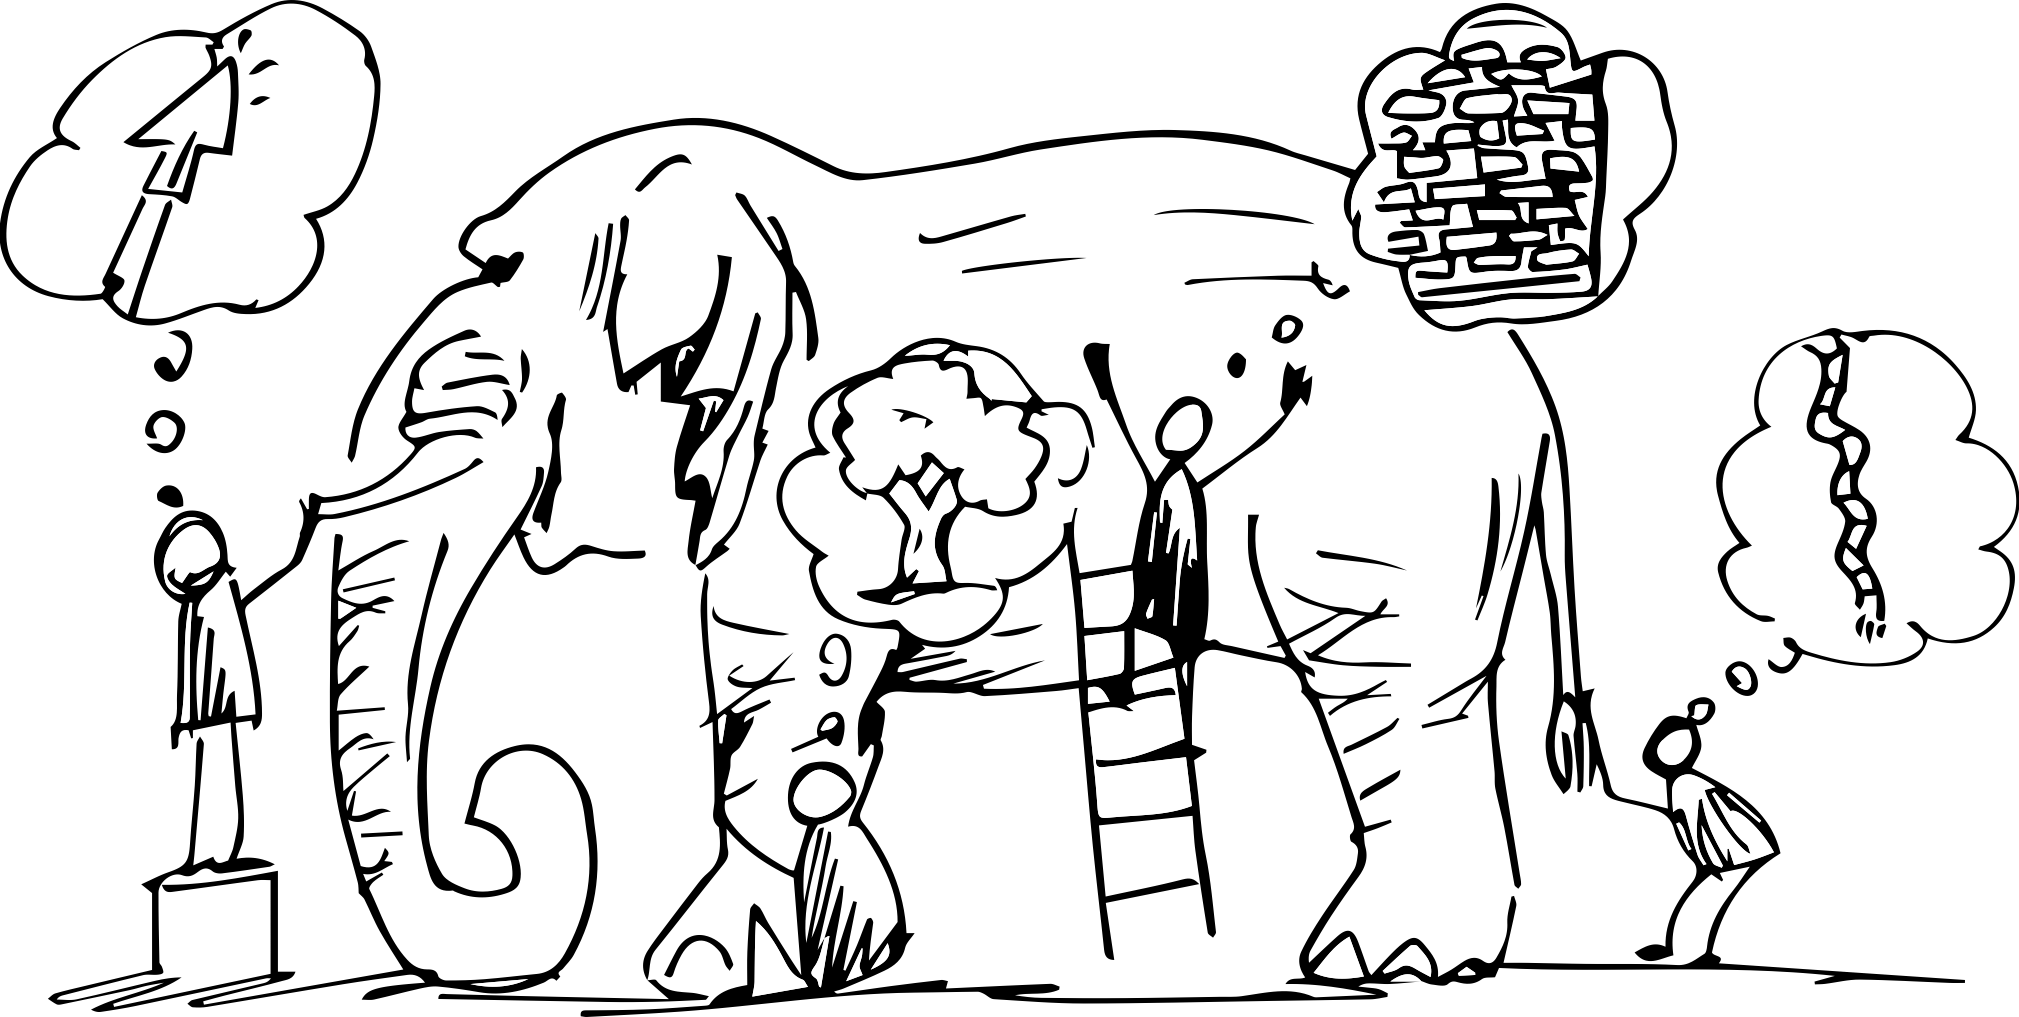
\includegraphics{imgs/elephant.png}

}

\caption{The Blind Men and the Elephant.}

\end{figure}

\begin{quote}
\emph{\hfill\break
It was six men of Indostan\\
To learning much inclined,\\
Who went to see the Elephant\\
(Though all of them were blind),\\
That each by observation\\
Might satisfy his mind\\
---John Godfrey Saxe,\\
\hspace*{0.333em}\\
The Blind Men and the Elephant~\protect\hypertarget{blind_men}{}{}\\
}
\end{quote}

\hypertarget{building-intelligent-agents}{%
\section{Building Intelligent
Agents}\label{building-intelligent-agents}}

\hypertarget{sec-anatomy_ia}{%
\subsection{Anatomy of intelligent agents}\label{sec-anatomy_ia}}

Like the blind men in the parable, an intelligent agent shall model her
understanding of Nature from limited sensory data.

\begin{figure}

{\centering 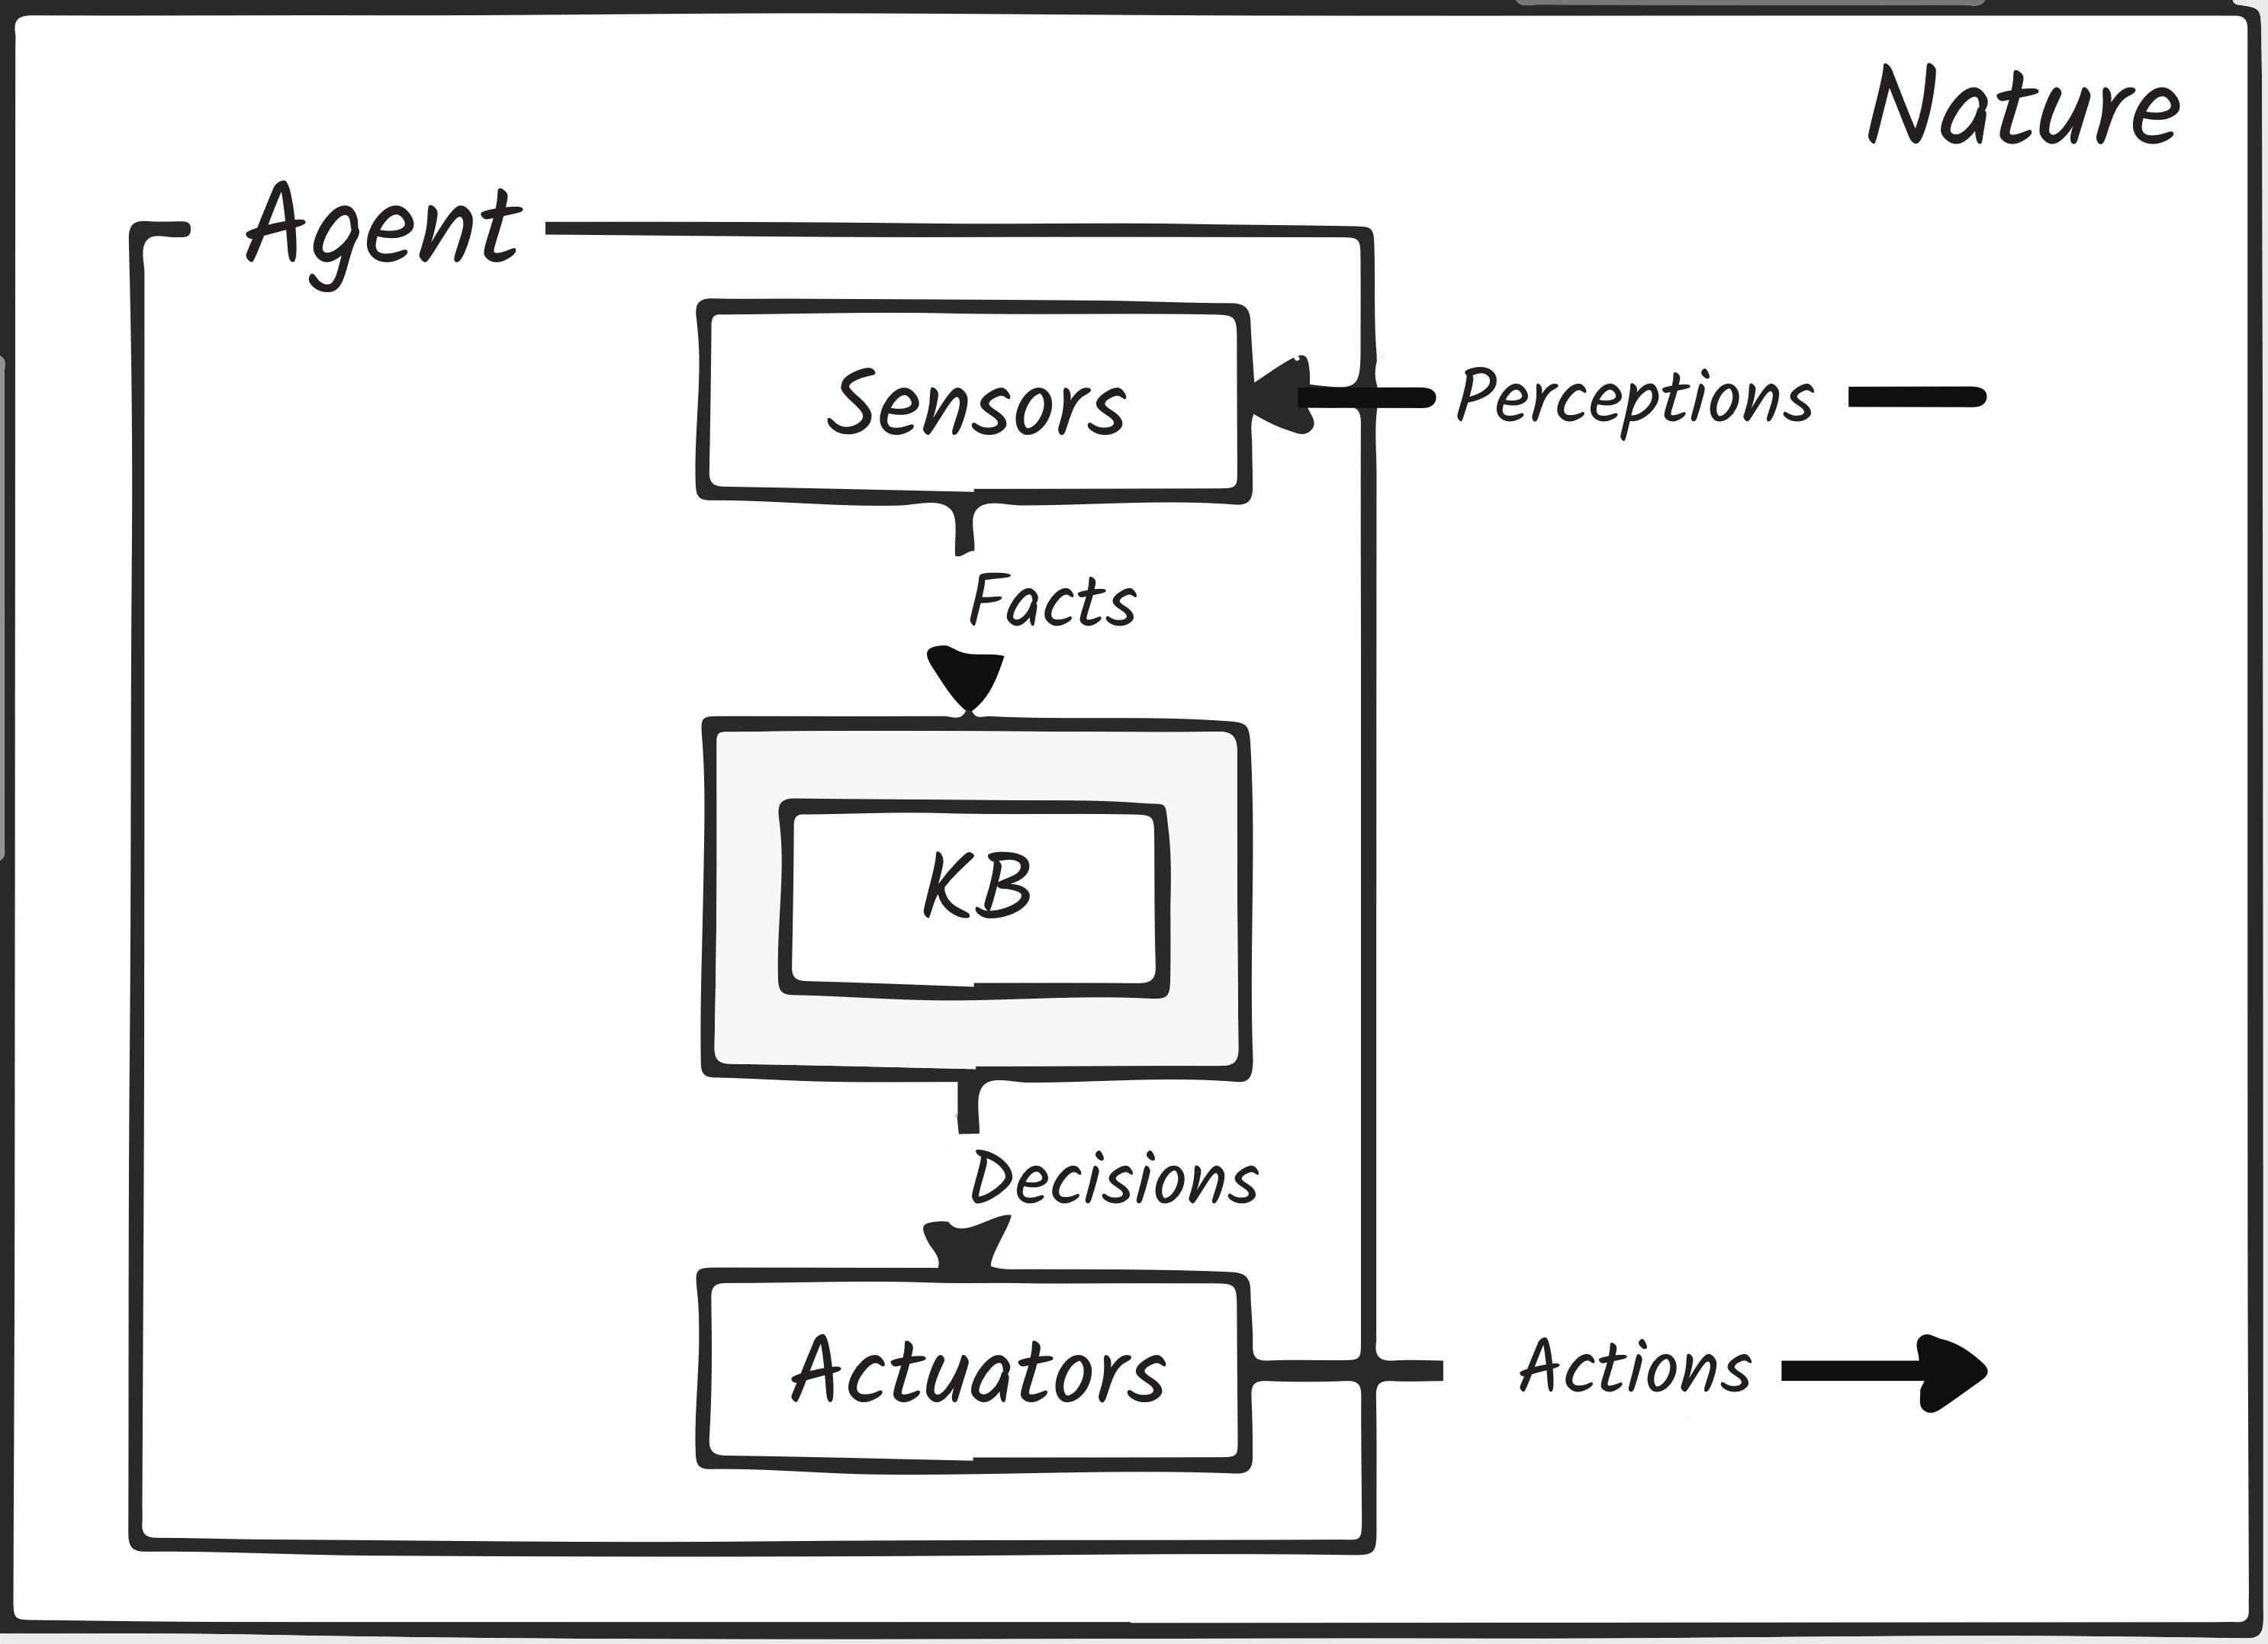
\includegraphics[width=0.6\textwidth,height=\textheight]{imgs/anatomy.png}

}

\caption{\label{fig-anatomy}Anatomy of an Intelligent Agent. Inspired by
art in ((\textbf{russell:2010?}))}

\end{figure}

Thus, an agent perceives her environment with sensors, treat sensory
data as facts and use these facts to possibly update her model of
Nature, use the model to decide her actions, and acts via her actuators.
In a way, agents continually communicate with Nature in a
perception/action conversation
(\protect\hyperlink{fig-anatomy}{{[}fig-anatomy{]}}).

The expected result of this conversation is a change in the agent's
{KB}, therefore in her model and, more importantly, her future
decisions. The model is an abstraction of how the agent ``thinks'' the
world is (her ``mental picture'' of the environment). Therefore, it
should be consistent with it: if something is true in Nature, it is
equally valid, \emph{mutatis mutandis}, in the model. A Model should
also be as simple as possible so that the agent can make decisions that
maximise a chosen performance measure, but not simpler. As the agent
knows more about Nature, less it gets surprised by it.

This rudimentary anatomy is flexible enough to entail different
epistemic views, like the rationalist (mathematical) and the empiricist
(scientific); different approaches to how to implement the knowledge
base (it can be learned, therefore updatable, or it can be set in stone
from an expert prior knowledge); and also from how to implement it (a
robot or software).

Noteworthy, though, is that the model that transforms input data into
decisions should be the target of our focus.

\hypertarget{symbolism}{%
\subsection{Symbolism}\label{symbolism}}

Symbolism is the pinnacle of rationalism. In the words of Thomas Hobbes,
one of the forerunners of rationalism, \emph{``thinking is the
manipulation of symbols and reasoning is computation''.} Symbolism is
the approach to building intelligent agents that does just that. It
attempts to represent knowledge with a formal language and explicitly
connects the knowledge with actions. It is \emph{competence from
comprehension}. In other words, it is \emph{programmed}.

Even though McCulloch and Pitts work on artificial neural networks
predates Von Neumann's computers, Symbolism dominated {AI} until the
\(1980\)s. It was so ubiquitous that symbolic {AI} is even called ``good
old fashioned AI''~(\textbf{russell:2010?}).

The symbolic approach can be traced back to Nichomachean
Ethics~(\textbf{aristotle:2000?}):

\begin{quote}
\emph{We deliberate not about ends but means. For a doctor does not
deliberate whether he shall heal, nor an orator whether he shall
persuade, nor a statesman whether he shall produce law and order, nor
does anyone else deliberate about his end. They assume the end and
consider how and by what means it is to be attained; and if it seems to
be produced by several means, they consider by which it is most easily
and best produced, while if it is achieved by one only they consider how
it will be achieved by this and by what means this will be achieved,
till they come to the first cause, which in the order of discovery is
last.}

--- Aristotle~
\end{quote}

This perspective is so entrenched that~(\textbf{russell:2010?}) still
says: \emph{``(\(\ldots\)) Only by understanding how actions can be
justified can we understand how to build an agent whose actions are
justifiable''}; even though, in the same book, they cover machine
learning (which we will address later in this chapter) without noticing
it is proof that there are other ways to build intelligent agents.
Moreover, it is also a negation of competence without comprehension. It
seems that even for AI researchers, the strange inversion of reasoning
is uncomfortable
(\protect\hyperlink{ch:introduction}{{[}ch:introduction{]}}).

All humans, even those in prisons and under mental health care, think
their actions are justifiable. Is that not an indication that we
rationalise our actions \emph{ex post facto}? We humans tend to think
our rational assessments lead to actions, but it is also likely possible
that we act and then rationalise afterwards to justify what we have
done, fullheartedly believing that the rationalisation came first.

\hypertarget{claude-shannons-theseus}{%
\subsubsection{Claude Shannon's Theseus}\label{claude-shannons-theseus}}

After writing what is probably the most important master's dissertation
of the 20\textsuperscript{th} century and ``inventing'' {IT}, what made
possible the Information Age we live in today, Claude Shannon enjoyed
the freedom to pursue any interest to which his curious mind led
him~(\textbf{soni:2017?}). In the \(1950\)s, his interest shifted to
building artificial intelligence. He was not a typical academic, in any
case. A lifelong tinkerer, he liked to ``think'' with his hand as much
as with his mind. Besides developing an algorithm to play chess (when he
even did not have a computer to run it), one of his most outstanding
achievements in AI was Theseus, a robotic maze-solving mouse.\sidenote{\footnotesize Many
  AI students will recognise in Theseus the inspiration to Russel and
  Norvig's Wumpus World~.}

To be more accurate, Theseus was just a bar magnet covered with a
sculpted wooden mouse with copper whiskers; the maze was the ``brain''
that solved itself~(\textbf{klein:2018?}).

\begin{quote}
\emph{``Under the maze, an electromagnet mounted on a motor-­powered
carriage can move north, south, east, and west; as it moves, so does
Theseus. Each time its copper whiskers touch one of the metal walls and
complete the electric circuit, two things happen. First, the
corresponding relay circuit's switch flips from''on'' to ``off,''
recording that space as having a wall on that side. Then Theseus rotates
\(90^{\circ}\) clockwise and moves forward. In this way, it
systematically moves through the maze until it reaches the target,
recording the exits and walls for each square it passes through.''
---~(\textbf{klein:2018?})}.
\end{quote}

\hypertarget{symbolic-ai-problems}{%
\subsubsection{Symbolic AI problems}\label{symbolic-ai-problems}}

Several symbolic AI projects sought to hard-code knowledge about domains
in formal languages, but it has always been a costly, slow process that
could not scale.

Anyhow, by \(1965\), there were already programs that could solve any
solvable problem described in logical notation~(\textbf{russell:2010?}).
However, hubris and lack of philosophical perspective made computer
scientists believe that ``intelligence was a problem about to be
solved\sidenote{\footnotesize Marvin Minsky, head of the artificial intelligence
  laboratory at MIT (\(1967\))}.''

Those inflated expectations lead to disillusionment and funding
cuts\sidenote{\footnotesize Sometimes called \emph{winters}.}~(\textbf{russell:2010?}).
They failed to estimate the inherent difficulty in slating informal
knowledge in formal terms: the world has many shades of grey. Besides,
complexity theory had yet to be developed: they did not count on the
exponential explosion of their problems.

\hypertarget{connectionism-a-different-approach}{%
\subsection{Connectionism: a different
approach}\label{connectionism-a-different-approach}}

The fundamental idea in Connectionism is that \textbf{intelligent
behaviour emerges from a large number of simple computational units when
networked together}~(\textbf{goodfellow:2016?}).

It was pioneered by McCulloch and Pitts in
1943~(\textbf{mcculloch:1943?}). One of Connectionism's first wave
developments was Frank Rosenblatt's Perceptron, an algorithm for
learning binary classifiers, or more specifically threshold functions:
\[\begin{aligned}
    y=
    \begin{cases}
        1 \text{ if } \mW\vx + \vb > 0\\
        0 \text{ otherwise }
    \end{cases}
\end{aligned}\] where \(\mW\) is the vector of weights, \(\vx\) is the
input vector, \(\vb\) is a bias, and \(\vy\) is the classification. In
neural networks, a perceptron is an artificial neuron using a step
function as the activation function.

\begin{figure}

\begin{minipage}[t]{0.50\linewidth}

{\centering 

\raisebox{-\height}{

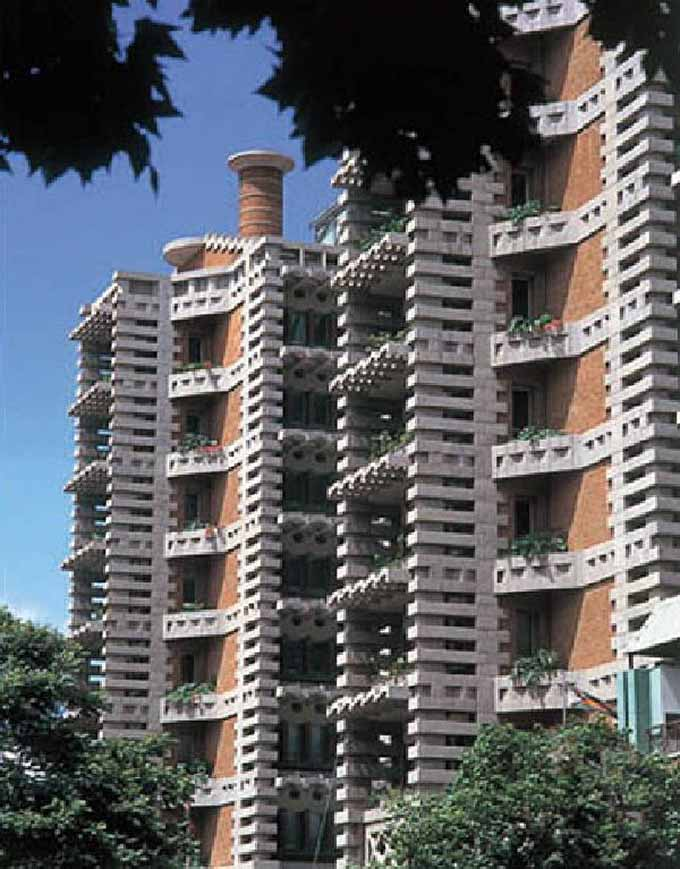
\includegraphics[width=2.60417in,height=\textheight]{imgs/arup_building.jpg}

}

\caption{\label{fig-arup_building}Building in Harare, Zimbabwe, modelled
after termite mounds. Photo by Mike Pearce.}

}

\end{minipage}%
%
\begin{minipage}[t]{0.50\linewidth}

{\centering 

\raisebox{-\height}{

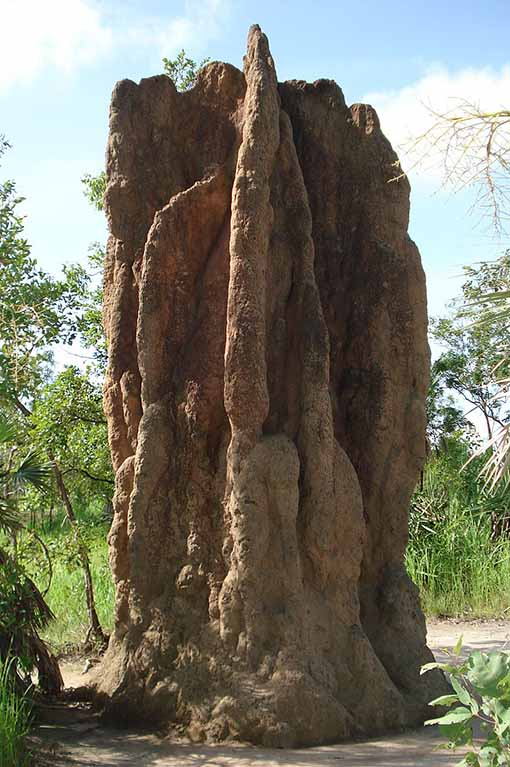
\includegraphics[width=2.60417in,height=\textheight]{imgs/termite_cathedral.jpg}

}

\caption{\label{fig-termite_cathedral}Cathedral termite mound,
Australia. Photo by Awoisoak Kaosiowa, 2008.}

}

\end{minipage}%
\newline
\begin{minipage}[t]{0.50\linewidth}

{\centering 

Biomimicry of termite technique achieves superior energy efficiency in
buildings.

}

\end{minipage}%

\end{figure}

See
\protect\hyperlink{fig-termite_cathedral}{{[}fig-termite\_cathedral{]}},
termites self-cooling mounds keep the temperature inside at exactly
\(31^{\circ} C\), ideal for their fungus-farming; while the temperatures
outside range from 2 to \(40^{\circ} C\) throughout the day. Such
building techniques inspired architect Mike Pearce to design a shopping
mall that uses a tenth of the energy used by a conventional building of
the same size.

From where does termites intelligence come?

\begin{quote}
\emph{Individual termites react rather than think, but at a group level,
they exhibit a kind of cognition and awareness of their surroundings.
Similarly, in the brain, individual neurons do not think, but thinking
arises in their connections.} --- Radhika Nagpal, Harvard
University~(\textbf{margonelli:2016?}).
\end{quote}

Such collective intelligence happens in groups of just a couple of
million termites. There are around 80 to 90 billion neurons in the human
brain, each less capable than a termite, but collectively they show
incomparable intelligence capabilities.

\begin{figure}

{\centering 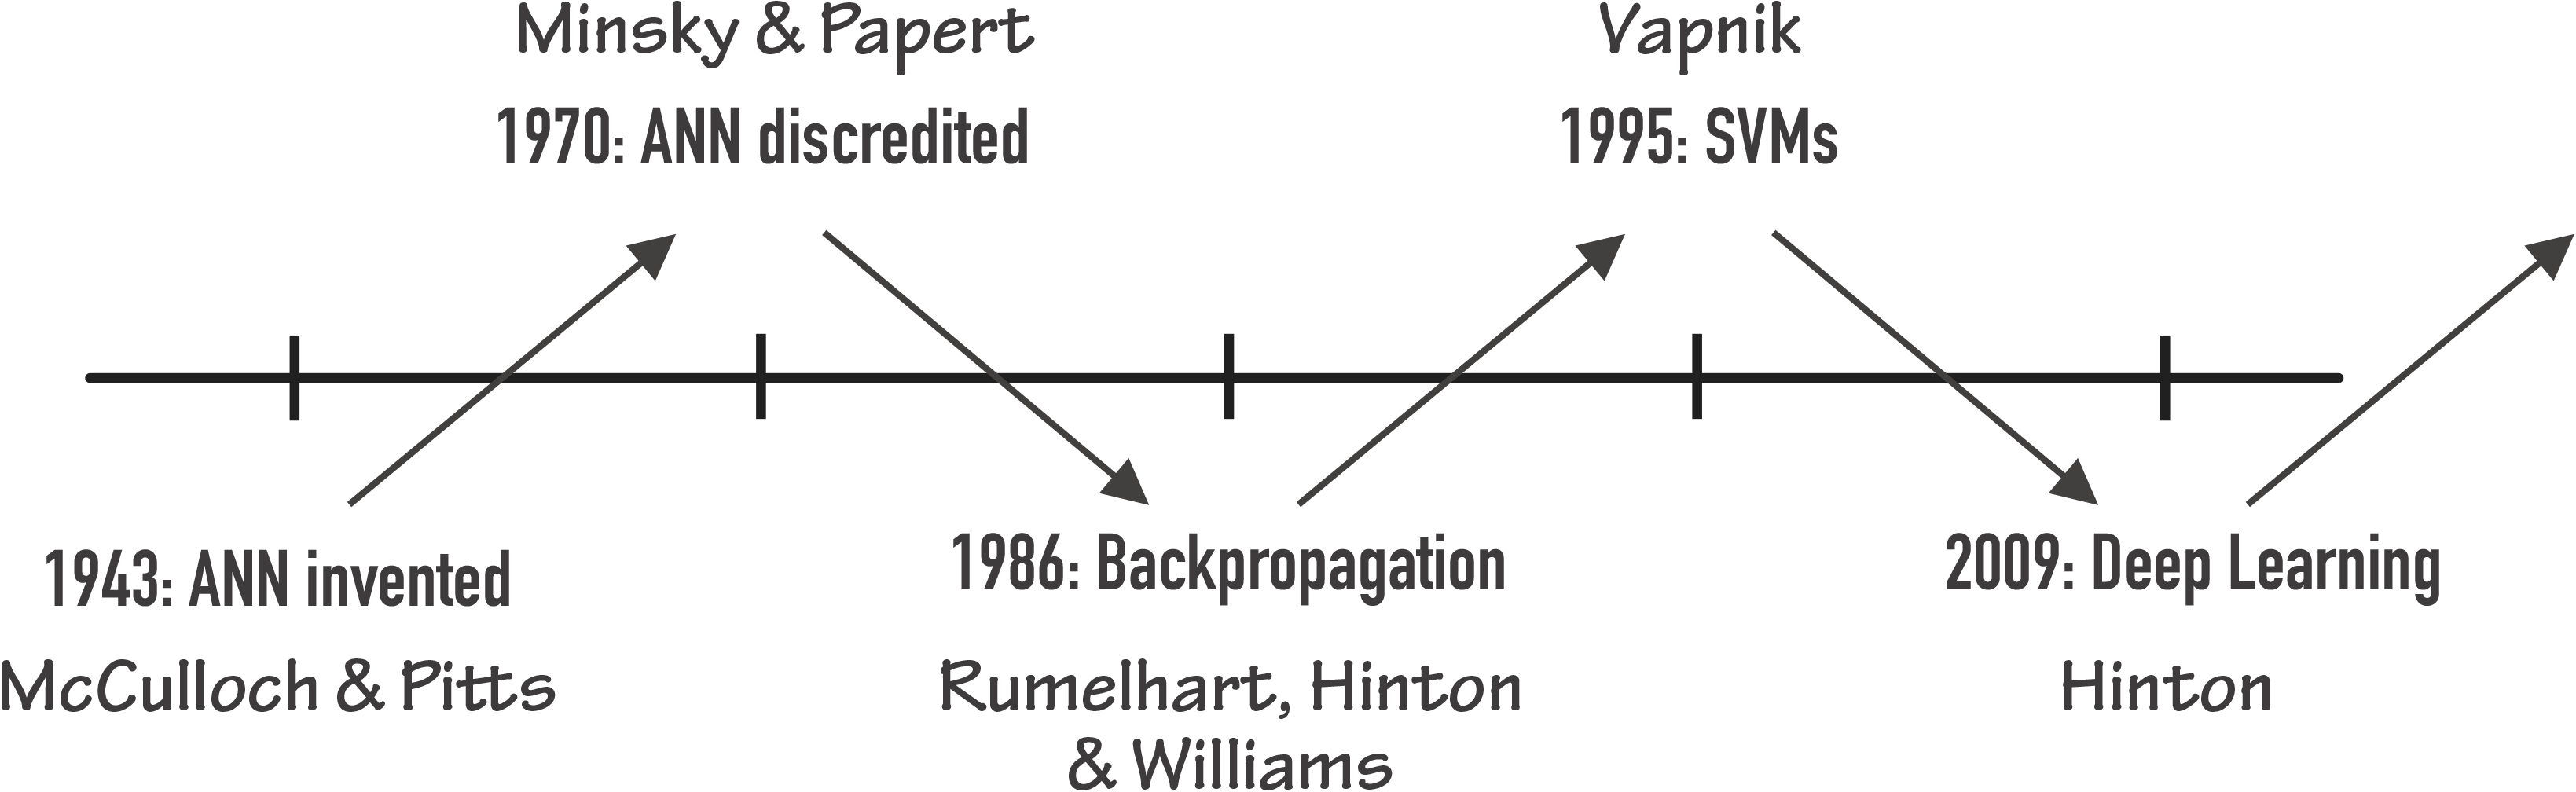
\includegraphics[width=0.8\textwidth,height=\textheight]{imgs/winters.png}

}

\caption{\label{fig-connectionism}A brief history of connectionism.
Adapted from ((\textbf{tishby:2020DeepMath?})).}

\end{figure}

In contrast with the symbolic approach, in neural networks, the
knowledge is not explicit in symbols but implicit in the strength of the
connections between the neurons. Besides, it is a very general and
flexible approach since these connections can be updated
algorithmically: they are algorithms that \emph{learn}: the
connectionist approach is an example of what we now call Machine
Learning.

\hypertarget{machine-learning}{%
\subsection{Machine Learning}\label{machine-learning}}

\begin{marginfigure}

{\centering 
\includegraphics{imgs/lulu.png}

}

\caption{\label{fig-lulu}Is this a cat?}

\end{marginfigure}

Look at \protect\hyperlink{fig-lulu}{{[}fig-lulu{]}}. Is this a picture
of a cat? How to write a program to do such a simple classification task
(cat/no cat)? One could develop clever ways to use \emph{features} from
the input picture and process them to guess. Though, it is not an easy
program to design. Worse, even if one manages to program such a task,
how much would it worth to accomplish a related \emph{task}, to
recognise a dog, for example? For long, this was the problem of
researchers in many areas of interest of AI:{CV}, {NLP}, Speech
Recognition {SR}; much mental effort was put, with inferior results, in
problems that we humans solve with apparent ease.

The solution is an entirely different approach for building artificial
intelligence: instead of making the program do the \emph{task}, build
the program that outputs the program that does the \emph{task}. In other
words, learning algorithms use ``training data'' to infer the
transformations to the input that generates the desired output.

\hypertarget{types-of-learning}{%
\subsubsection{Types of learning}\label{types-of-learning}}

Machine Learning can happen in different scenarios, which differ in the
availability of training data, how training data is received, and how
the test data is used to evaluate the learning. Here, we describe the
most typical of them~(\textbf{mohri:2012?}):

\begin{itemize}
\item
  \textbf{Supervised learning:} The most successful scenario. The
  learner receives a set of labelled examples as training data and makes
  predictions for unseen data.
\item
  \textbf{Unsupervised learning:} The learner receives unlabelled
  training data and makes predictions for unseen instances.
\item
  \textbf{Semi-supervised learning:} The learner receives a training
  sample consisting of labelled and unlabelled data and makes
  predictions for unseen examples. Semi-supervised learning is usual in
  settings where unlabelled data is easily accessible, but labelling is
  too costly.
\item
  \textbf{Reinforcement learning:} The learner actively interacts with
  the environment and receives an immediate reward for her actions. The
  training and testing phases are intermixed.
\end{itemize}

\hypertarget{deep-learning}{%
\subsection{Deep Learning}\label{deep-learning}}

The \(2010\)s have been an AI Renaissance not only in academia but also
in the industry. Such successes are mostly due to {DL}, in particular,
supervised deep learning with vast amounts of data trained in {GPUs}. It
was the decade of {DL}.

\begin{quote}
\emph{``Deep learning algorithms seek to exploit the unknown structure
in the input distribution to discover good representations, often at
multiple levels, with higher-level learned features defined in terms of
lower-level features.'' --- Joshua Bengio~(\textbf{bengio:2012?})}
\end{quote}

The name is explained by ~(\textbf{goodfellow:2016?}): ``\emph{A graph
showing the concepts being built on top of each other is a deep graph.
Therefore the name, deep learning}''~(\textbf{goodfellow:2016?}).
Although it is a direct descendant of the connectionist movement, it
goes beyond the neuroscientific perspective in its modern form. It is
more a general principle of learning multiple levels of compositions.

The quintessential example of a deep learning model is the deep
feedforward network or {MLP}~(\textbf{russell:2010?}).

Let,

\begin{itemize}
\item
  be the input vector \(\{\vx_1, \ldots, \vx_m\}\)
\item
  be the layer index, such that \(k \in [1,l]\),
\item
  be the matrix of weights in the \(k\)-th layer, where
  \(i \in [0,d_{k-1}], j \in [1, d_k] \text{ and }\mW^{(k)}_{0,:}\) are
  the biases
\item
  be a nonlinear function,
\end{itemize}

a \textbf{{MLPs}} is a neural network where the input is defined by:
\$\$

\begin{aligned}
        h^{(0)}= 1^\frown \vx,
    
\end{aligned}

\[ a hidden layer is defined by: \]

\begin{aligned}
        h^{(k)}&=\sigma^{(k)}(\mW^{(k)~\top} h^{(k-1)}).
    
\end{aligned}

\[ The output is defined by: \]

\begin{aligned}
        \hat{y}&=h^{(l)}.
    
\end{aligned}

\$\$

Deep Learning is usually associated with {DNNs}, but the network
architecture is only one of its components:

\begin{enumerate}
\def\labelenumi{\arabic{enumi}.}
\item
  DNN architecture
\item
  {SGD} --- the optimiser
\item
  Dataset
\item
  Loss function
\end{enumerate}

The architecture is not the sole component essential to current Deep
Learning success. The {SGD} plays a crucial role, and so does the usage
of large datasets.

A known problem, though, is that DNNs are prone to overfitting
(\protect\hyperlink{sec-bias-variance}{{[}sec-bias-variance{]}}).
~(\textbf{zhang:2016?}) show state-of-the-art convolutional deep neural
networks can easily fit a random labelling of training
data~(\textbf{zhang:2016?}).

\hypertarget{concluding-remarks}{%
\section{Concluding Remarks}\label{concluding-remarks}}

This chapter derived the need for a \emph{language} from the definitions
of \emph{intelligence} and \emph{intelligent agents}. An intelligent
agent needs \emph{language} to store her knowledge (what she has
learned) and with that to communicate/share this knowledge with its
future self and with other agents.

We claim (without proving) that a language can be derived from a
definition of knowledge: an epistemic choice. We claim that mathematics
and science can be seen as languages that differ in consequence of
different views on what knowledge is and gave historical background on
two epistemic views, Rationalism and Empiricism
(\protect\hyperlink{sec-rationalismux2csec-empiricism}{{[}sec-rationalism,sec-empiricism{]}}).

We gave historical background on {AI} and showed that different
epistemic views relate to {AI} movements: Symbolism and Connectionism.
We gave some background on basic {AI} concepts: intelligent agents,
machine learning, types of learning, neural networks and deep learning,
showing that {DL} relates to Connectionism and, hence, to science and an
empiricist epistemology. Previously
(\protect\hyperlink{sec-bringing_science}{{[}sec-bringing\_science{]}}),
we have discussed that Computer Science generally relates to the
rationalist epistemology. We hope this can help us better understand our
research community.

\hypertarget{assumptions}{%
\subsection{Assumptions}\label{assumptions}}

\begin{enumerate}
\def\labelenumi{\arabic{enumi}.}
\item
  A definition of intelligence
  (\protect\hyperlink{def-intelligence}{{[}def-intelligence{]}})
\item
  An epistemic choice on the definition of Knowledge
  (\protect\hyperlink{sec-rationalismux2csec-empiricism}{{[}sec-rationalism,sec-empiricism{]}})
\end{enumerate}



\end{document}
